\section{\acrlong{clt}} \label{sec:bt/CLT}

\acrfull{clt} as a field of study was first developed by \textcite{sweller1988} as a means of optimizing intellectual performance in learning environments. By categorizing differing levels of strain imposed on the user in various problem solving tasks, he was able to reason between the efectiveness of different formats of information presentation for learning. He elaborates his theories a decade later, in a paper outlining a system for human cognitive architecture. With this system, he provided tools to describe the nature of mental processing demands, intellectual skill and the ability to learn.

% automaticity of long-term memory, as well as the ability to free up working memory in order to effectively learn and master unknown tasks.

% The role of cognitive load in instructional design.

\subsection{What is Cognitive Load?}

% "Cognitive load, a multidimensional construct, represents the load that performing a particular task imposes on the cognitive system". This definition by \textcite{paas1994} encapsulates the broad nature of cognitive load, in relation to a particular task. 

Cognitive load is a broad term aimed at describing the load imposed on the cognitive system while performing a particular task \cite{paas1994}. Considering the complex nature of the cognitive system, and all factors both affecting and affected by cognitive load, the term is necessarily very comprehensive. To fully understand the nature of cognitive load, we need to describe it in terms of its defining factors. 

One such factor is the distinction between \textit{mental load}, \textit{mental effort} and \textit{performance}. Although similar on the surface, these three dimensions are the cause for much difficulty when cognitive load is to be assessed.

Consider the case of one participant in an experimental trial where researchers want to measure cognitive load. The participant is presented with one or more tasks, each with varying levels of difficulty. Each task is then said to impose a mental load, and the amount of cognitive resources the participant actually allocates to perform this task is defined as mental effort \cite{paas1994}. Whereas mental effort is dynamically determined by the cognitive control and focus of the participant, mental load will be constant with every task. Furthermore, when researchers want to measure the cognitive load imposed, a performance metric is often employed. Although there is a clear relationship between high cognitive load and low performance, performance measures may in practice show little deficits with increasing task demands because the participant is able to invest more mental effort to compensate for increasing mental load \cite{tulga1980}.

Consequently, the intensity of effort expended (mental effort) is often considered the essense of cognitive load \cite{hamilton1979}, since this metric may yield important information that is not necessarily reflected in performance-based measures. Even so, the measurement of mental effort is no trivial task, and have long been dependent on inaccurate indices of subjective self-assessment. Given the fact that changes in cognitive functioning often are reflected in physiology, later years have seen the emergence of more objective physiological measures. Some such measures are based on pupillary diameter, eyeblink rate and more, for reasons to be detailed in section \ref{sec:bt/cognitive_impacts}.

\subsection{Three Domains of \acrlong{clt}}

% Another defining factor of cognitive load besides assessment, is dependent on the participant. This factor is relatively stable and not likely to change during the course of the task, such as cognitive capabilities and prior knowledge.

% Upon receiving sensory input, any information processing is initially done in working memory. The degree of which this task is considered difficult or straining depends on the imposed cognitive load, which is determined by several factors. 

Central to human cognitive architecture is the capacity of working memory and the relative load imposed by incoming information. \textcite{sweller1988} proposed a system similar to figure \ref{fig:bt/information_processingA} to describe the typical flow of information in the human information processing system. As is apparent from the figure, there is a constant interplay of information to and from working memory, which is where both incoming and encoded information is processed for all intents and purposes. The ease of which information may be processed in working memory is a prime consern of \acrshort{clt}, and is often condensed into three domains.

\begin{figure}[h]
    \begin{subfigure}[b]{\textwidth}
        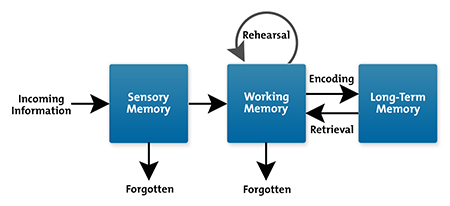
\includegraphics[width=0.9\textwidth]{figures/bt_information_processingA.jpg}
        \caption{Intuitive presentation of the information processing system.}
        \label{fig:bt/information_processingA}
    \end{subfigure}
    \begin{subfigure}[b]{\textwidth}
        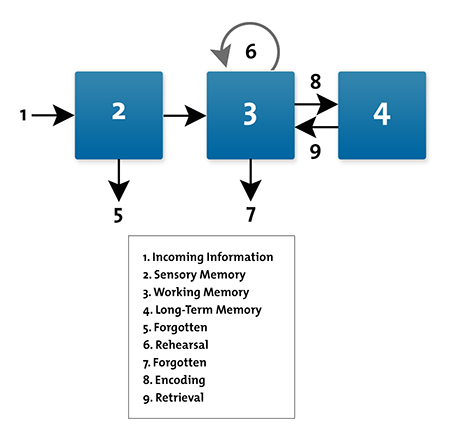
\includegraphics[width=0.9\textwidth]{figures/bt_information_processingB.jpg}
        \caption{Less intuitive presentation of the information processing system.}
        \label{fig:bt/information_processingB}
    \end{subfigure}
    \caption{Example of how two presentations of the same information impose different levels of extraeneous cognitive load.}
    \source{\cite{mindtools2016}}
\end{figure}

First, the information presented can be intrinsically hard to process, often due to a high level of element interactivity. The more elements that need to be kept in memory at one time, the higher the mental load. As an example, the process of learning a new language by memorizing individual words has a low level of element interactivity, since only a pair of words need to be kept in memory in order to learn their association. In contrast, learning a language also requires grammatical knowledge. In this case, relationships in entire sentences requires multiple words and meanings to be kept in memory at one time, and hence represents a high level of element interactivity. Cognitive load imposed by the underlying nature of the information is called \textit{intrinsic cognitive load}.

On top of the intrinsic cognitive load imposed by the information itself, is its \textit{extraneous cognitive load}. This domain depends on the way in which information is presented, whether intuitively or unintuitively. Consider for example the presentations of figure \ref{fig:bt/information_processingA} compared to figure \ref{fig:bt/information_processingB}. Clearly, they represent the same information and hence impose the same intrinsic cognitive load. Yet, the second figure places higher demands on working memory by forcing the viewer to memorize labels, and is therefore more difficult to process. Extraneous congitive load is understandably a fundamental concern when designing learning environments, where one can choose between presentation formats. One generally wants the extraenous cognitive load to be as low as possible in order to optimize learning, and make room in working memory for what is known as \textit{germane cognitive load}.

Within human cognitive architecture, \textcite{sweller1988} establishes that learning and understanding is simply the encoding of complex information and relationships so that it can effectively be stored in long-term memory. Information is compressed into frameworks of understanding called \textit{schemas}. When such information is later encountered anew, this understanding is decoded from memory for reuse. For instance, when fresh mathematicians are to learn to multiply out the denominator in an equation such as $a/b=c$, they have to hold several concepts in working memory. For one, they need to know that $b$ can be multiplied onto both sides of the equation without affecting $a$. Second, the concept that $b/b=1$ must be readily known, and third that $a*1=a$. For someone that has no prior knowledge of algebra, this is a problem with high element interactivity, and likely demands high cognitive load to solve. A learned student, however, can merely shift $b$ to the right to give $cb$. Learning the procedure in this way substantially reduces the cognitive load at the expense of prior understanding.

Germane cognitive load is the load imposed on working memory from constructing these schemas. When designing learning environments, \textcite{sweller1988} therefore recommends that "the learner's attention must be withdrawn from processes not relevant to learning and directed toward processes that are relevant to learning and, in particular, toward the construction and mindful abstraction of schemas". As an example, a student is much more prone to understand a complex topic through intructional procedures such as asking questions about an example, rather than memorizing their solutions directly. By encouraging the student to engage in the topic, concious effort in working memory will be made to create topic understanding. 

In summary, master chess players experience less cognitive load from a chess game than a novice, and a professor might consider an example trivial while students scratch their head in confusion. This is not to say that the expert chess player or professor necessarily have a much higher cognitive capacity than the novice, but rather that they possess a heightened understanding. Understanding comes in the form of compressed schemas in long-term memory, which allows topics to demand much less intrinsic cognitive load when recalled. Experience has been acquired though years of concious effort, likely with high germane cognitive load imposed on working memory.

\subsection{Working Memory, Long-term Memory and Intelligence}
\textit{Describe Sweller's theory on working memory, long-term memory, schema contruction, intelligence and ability to learn. Maybe mention parallell to Kahneman's "Thinking, Fast and Slow"}

\FloatBarrier